%% This is a skeleton file demonstrating the use of IEEEtran.cls (requires IEEEtran.cls version 1.8a or later) with an IEEE conference paper.
%%
%% Modified by Khan Reaz( kahn.reaz@ieee.org)
%% Support sites:
%% http://www.ieee.org/

%%***********************************************************
%% Legal Notice:
%% This code is offered as-is without any warranty either expressed or implied; without even the implied warranty of MERCHANTABILITY or FITNESS FOR A PARTICULAR PURPOSE! 
%% User assumes all risk and can modify as s/he wants.

%%***********************************************************

%package list
\documentclass[conference]{IEEEtran}
\usepackage{cite}
\usepackage{graphicx}
\graphicspath{ {images/} }
\usepackage[brazil]{babel}
\usepackage[utf8]{inputenc}

\begin{document}

\title{Análise de classificadores}
\author{Aryane Ast dos Santos}


%Authors List

\author
{\IEEEauthorblockN{Aryane Ast dos Santos}
\IEEEauthorblockA{Departamento de Informática\\
Universidade Federal do Paraná\\
Email: aras10@inf.ufpr.br}
}

\maketitle


%Main body starts

%\begin{abstract}
%Abstract goes here

%\end{abstract}


%\begin {cIEEEkeywords}
%
%IoT, Ontology, Semantics,  SSN, OWL, OBOE, OpenIoT, SWEET, SUMO
%\end{IEEEkeywords}


\section{Introdução}

Um problema de classificação consiste em definir um rótulo ou classe para um
elemento a partir de um conjunto de elementos com rótulos definidos. É um
problema de aprendizagem supervisionada, cujo objetivo é realizar inferências a
partir de um conjunto de dados rotulados, em oposição à aprendizagem
não-supervisionada.

Este relatório se propõe a apresentar resultados obtidos com os
classificadores \emph{K Nearest Neighbors} (KNN), \emph{Naive Bayes}, Árvores de
Decisão e \emph{Support Vector Machines} (SVM) para um problema de classificação de
imagens, cuja base rotulada possui 1901 imagens divididas 9 classes diferentes.
Os algoritmos de classificação não utilizam as imagens "brutas", sendo necessário, então, converter as imagens do formato JPG para vetores de características
que os algoritmos de classificação possam utilizar.

Após extraído os vetores de características das imagens, foram realizadas
as execuções dos classificadores KNN, Naive Bayes, Árvores de Decisão e SVM. As
implementações dos algoritmos mencionados são da biblioteca Scikit Learn (ref).

Nas seções a seguir são apresentados maiores detalhes da representação,
algoritmos utilizados, métricas para comparação e desempenho.
São comparados também o desempenho de estratégias de combinação de
classificadores e \emph{ensembles}.

\section{Representação dos dados}

Para cada uma das imagens disponibilizadas para classificação, é realizada uma
extração de características, que resulta num vetor com as características

Para a extração dos vetores de caracteristicas, foram utilizados os algoritmos
\emph{Local Binary Patterns} (LBP) e \emph{Grey-Level Co-Occurrence Matrix}
(GLCM), o que resultou em vetor contendo 24 características, além da classe ao
final da linha.

\subsection{Local Binary Patterns}
Breve explicação. Método uniforme, raio=2, n\_point ou vizinhos = 16,
implementação do scikit learn.

\subsection{Grey-Level Co-Occurrence Matrix}

Breve explicação.

Características utilizadas: correlação, dissimilarity, contrast, homogeneity,
energy, ASM.
%http://scikit-image.org/docs/dev/api/skimage.feature.html#skimage.feature.greycoprops

\section{Classificação}

A partir dos vetores de características, é possível executar os
algoritmos de classificação. Como temos apenas uma base de dados, se a
utilizarmos inteira para treinar os algoritmos e após isso, testar se a
classificação é feita corretamente com essa mesma base, ocorrerá algo chamado de
\emph{overfitting}, que ocorre quando a base é muito especializada e acerta predições
para um conjunto de dados conhecido, mas para dados desconhecidos costuma errar.
Para fugir dessa situação, é boa prática separar a base em treinamento e
validação.

Entretanto, ao separar a base em treinamento e validação, reduz-se muito a
quantidade de dados dos quais se aprende (dados treinamento). Para evitar tal
situação, se faz uso de uma técnica chamada validação cruzada ou
\emph{cross-validation}, onde se separa ...

Neste trabalho, para a validação cruzada são utilizados os métodos ShuffleSplit
e cross\_val\_score do módulo model\_selection da biblioteca SciKit Learn. Dessa
forma, a base é dividida 10 vezes em treinamento e validação nas proporções de
0.6 e 0.4 respectivamente.

\subsection{Métricas}

Precisão é a abilidade de um classificador não rotular com positivo uma amostra
que é negativa. Recall é a abilidade do classificador de encontrar todas as
amostras positivas. Já a métrica F-measure podem ser interpretadas como médias
harmônicas da precisão e recall.


\subsection{KNN}

O KNN (K-Nearest Neighbors) classifica um dado x atribuindo a ele o rótulo
representado mais frequentemente dentre as k amostras mais próximas. O
algoritmo recebe apenas um parâmetro: o inteiro k. Variando k de 3 a 30, foi
possível perceber que o k que propocionou melhor média de acurácia dentre os 10
folds de validação cruzada foi 5. A média de acurácia foi de 0,51 com margem de
erro de 0,01.


\subsection{Naive Bayes}

Naive Bayes é um método que utiliza uma abordagem probabilística para a
aprendizagem supervisionada ao aplicar o Teorema de Bayes ao problema. É
considerado ingênuo (naive) por assume independência entre as características.


\subsection{Árvores de decisão}

Breve explicação


\subsection{SVM}

O classificador do SVM (Support Vector Machines) encontra um hiperplano de
separação para dados de duas classes distantas. Busca-se maximizar a distância
entre o hiperplano e os dados de treinamento, e à essa distância é dado o nome
margem.

Apesar de o SVM ser um classificador linear binário, a maioria dos
problemas não possuem apenas duas classes nem são linearmente separáveis, seja
pela ocorrência de outliers, mas na maioria dos casos é pela própria
distribuição dos dados.

Ainda assim, o SVM se mostra apropriado para ser utilizado em tais casos. Com o
Kernel Trick, é possível projetar os dados em um espaço onde eles são
linearmente separáveis. E para resolver o problema de várias classes, existe a
estratégia de um-contra-todos (one-versus-rest), onde se n é o número de
classes, são treinados n classificadores que utilizam os dados de uma das
classes contra os dados de todas as outras juntas, obtendo assim n
classificadores lineares.


\section{Ensembles}

\subsection{Random forests}

Random forests funcionam como uma coleçao de árvores de decisão não
relacionadas entre si.

Possui dois parâmetros principais, o número de estimadores n\_estimators e
número máximo de features max\_features. O número de estimadores define a
quantidade de árvores de decisão da floresta. Intuitivamente, quando mais
árvores, melhor o resultado, apesar de levar mais tempo para executar o
algoritmo. Porém, ao executar o classificar para números de estimadores
variando entre 10 e 100, foi possível observar que a média de acurácia, pois se
trabalhou com validação cruzada, foi de 0,79, com tolerância de 0,01 para
números de estimadores a partir de 59 até 100. E como o algoritmo roda muito
mais rápido com um número menor de árvores, 59 foi o n\_estimatores escolhido.

Já o parâmetro max\_features se refere à quantidade de características
utilizadas. De acordo com a documentação do SciKit-Learn, max\_features como
raiz quadrada do número de características gera bons resultados, que neste caso
seria próximo de 5. Obtive as melhores médias de acurácia para max\_depth
variando de 5 a 19.

\section{Teste de Wilcoxon}

O teste de Wilcoxon é um teste de hipóteses que 

\section{Considerações Finais}

Podemos perceber que.
Todo o código utilizado no projeto, inclusos ..., pode ser encontrado num
repositório Git hospedado no GitHub ....

%\section{Introduction}
%\label{intro}
%Here goes the introduction
%
%%example for Bullet point list
%
%\begin{itemize}
%\item example
%\end {itemize}
%
%%example for numbered list
%    \begin{enumerate}
%    \item example
%    \end{enumerate}
%
%%example for inserting image
%\begin{figure}[h]
%   \centering
%   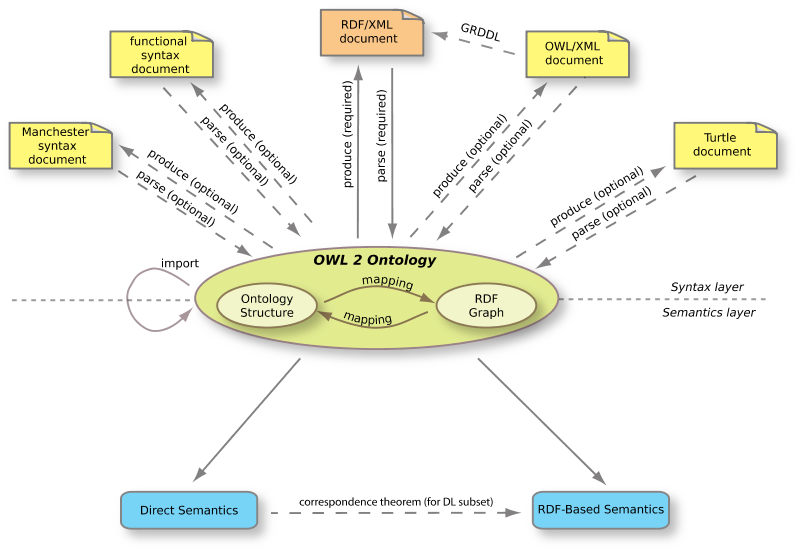
\includegraphics[scale=.45]{OWL2}
%    \caption{The structure of OWL2}
%    \label{fig:OWL2}
%\end{figure}
%
%\section{Conclusion}
%\label {conclusion}
%\input{sections/5_conclusion.tex}
%
%\bibliographystyle{IEEEtran}
%\bibliography{bibliography}

\end{document}
